\section{Introduction}	
% Explanation of title and why someone should read
This paper introduces an algorithm to be used for indoor painting detection and localization applied to the frames of a video sequence. To achieve this goal we have constructed an algorithm that attempts to efficiently match detected paintings from a stream of images and to localize it on a ground plan.

% Contributions
This paper contains three contributions which will be discussed more in depth in the following section.


Our first contribution of this paper is a method for segmenting a given image or a video frame into a painting with its frame and the rest of the picture. This extracted painting is transformed to a standard format which serves as an input to our other contribution . It is inspired by the works of Canny (1986) \cite{Canny1986} and Suzuki et al. (1985) \cite{SUZUKI198532} and combines them to allow robust approximation of a polygon and its extraction from the source material \todo{need paper, check wiki}.


The second contribution of this paper is a robust algorithm for matching an extracted painting with an existing database of paintings. It is inspired by the works of Rublee et al. (2011) \cite{Rublee2011} which uses Brute Force matching based on ORB and should be more efficient than the existing work of Lowe (1999) \todo{check and add to library}.


The final contribution of this paper is the usage of meta-data associated with the matched painting from the database. In our implementation, the meta-data is used to provide a strict way of localizing the painting and, by extension, the user on a floor plan (or its graph counterpart). The algorithm is not limited by this meta-data in its current state, as it can be expanded should the need arise.

% Results
The database of 688 paintings is matched every 50 frames with the videos running at 30 frames per second. All paintings are compressed to 1000 x 1000 pixels in order to speed up the matching procedure. In order to test the efficiency of our algorithm, a ground truth was established by taking a small sample of 30 paintings and manually labeling them. We achieved a segmentation accuracy of 88.57\% and a painting matching accuracy and subsequently localization accuracy of 47.10\%.

% Usefulness
This algorithm can have practical uses beyond the detection of paintings. As this method may be used in a similar fashion for detecting other types of objects or localizing a user in a different museum. This method is also viable for implementation on a smartphone where users may receive additional information on the painting or the room that they are localized in. Again the user must not be specifically located in a museum for this method to work as the database that the method builds upon can be exchanged between different runs of the algorithm.

\subsection{Overview}
The succeeding sections of this paper will discuss the implementation of the proposed algorithm. Section \ref{sec:painting_detection} will discuss the inner workings of the algorithm. Section \ref{sec:results} will describe the used performance metrics to evaluate the effectiveness of the algorithm, the experimental results and finish it up by presenting a qualitative analysis where the strengths and weaknesses of our proposed algorithm are laid bare.



\begin{figure}
	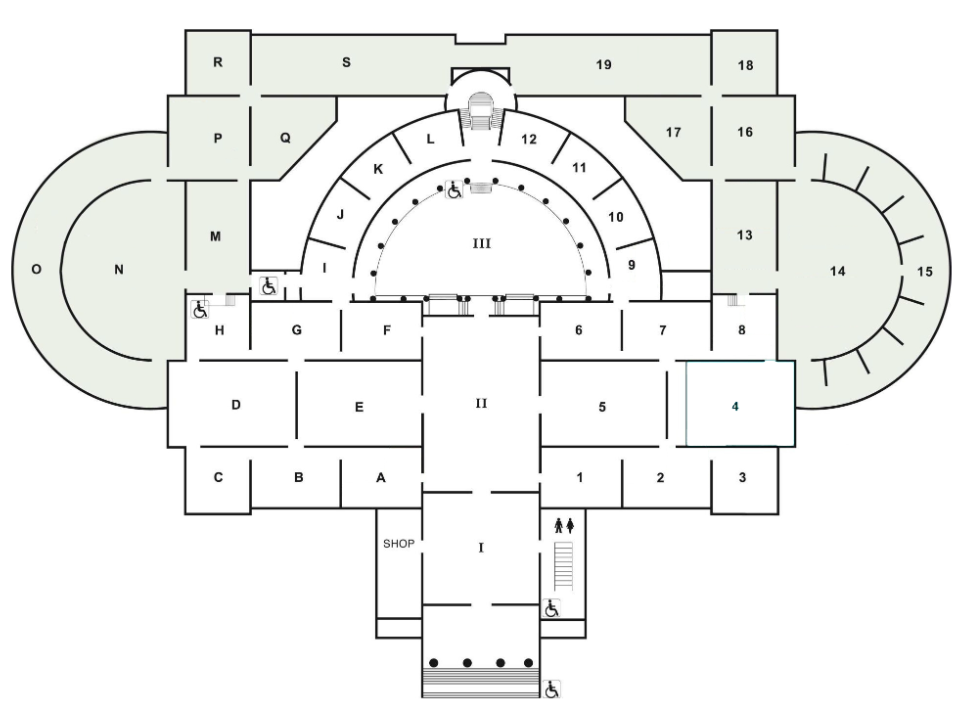
\includegraphics[width=\linewidth]{groundplan_msk}
	\caption{A ground plan of The Museum of Fine Arts, Ghent. }
	\label{fig:groundplan_msk}
\end{figure}